\documentclass{tufte-handout}

\title{Section 5.1: The Unit Circle}

\author[AW]{Ammon Washburn}

\usepackage{graphicx} % allow embedded images
  \setkeys{Gin}{width=\linewidth,totalheight=\textheight,keepaspectratio}
  \graphicspath{{graphics/}} % set of paths to search for images
\usepackage{amsmath}  % extended mathematics
\usepackage{booktabs} % book-quality tables
\usepackage{units}    % non-stacked fractions and better unit spacing
\usepackage{multicol} % multiple column layout facilities
\usepackage{lipsum}   % filler text
\usepackage{enumerate}
\usepackage{wrapfig}
\usepackage{fancyvrb} % extended verbatim environments
  \fvset{fontsize=\normalsize}% default font size for fancy-verbatim environments
\usepackage{tikz}
\usepackage{subcaption}
\captionsetup{compatibility=false}
\usepackage{mathtools}
\usepackage{graphicx}
\usepackage{amssymb}
\usepackage{enumerate}
\usepackage{color}
\usepackage{fancyvrb}
\usepackage{breqn}
\usepackage{fancyhdr}
\usepackage{multicol}
%\usepackage[latin1]{inputenc}
\usepackage{tikz}
\usepackage{pgfplots}
\pgfplotsset{compat=1.8}

\definecolor{dkgreen}{rgb}{0,0.6,0}
\definecolor{gray}{rgb}{0.5,0.5,0.5}
\definecolor{mauve}{rgb}{0.58,0,0.82}

\newcommand{\R}[1]{\mathbb{R}^{#1}}

\pgfplotsset{vasymptote/.style={
    before end axis/.append code={
        \draw[densely dashed] ({rel axis cs:0,0} -| {axis cs:#1,0})
        -- ({rel axis cs:0,1} -| {axis cs:#1,0});
    }
}}
\pgfplotsset{hasymptote/.style={
    before end axis/.append code={
    	%\draw (axis cs:0,1) -- ({axis cs:0,1}-|{rel axis cs:1,0});
        \draw[densely dashed] ({rel axis cs:0,1} -| {axis cs:0,#1})
        -- ({rel axis cs:0,0} -| {axis cs:0,#1});
    }
}}

% Standardize command font styles and environments
\newcommand{\doccmd}[1]{\texttt{\textbackslash#1}}% command name -- adds backslash automatically
\newcommand{\docopt}[1]{\ensuremath{\langle}\textrm{\textit{#1}}\ensuremath{\rangle}}% optional command argument
\newcommand{\docarg}[1]{\textrm{\textit{#1}}}% (required) command argument
\newcommand{\docenv}[1]{\textsf{#1}}% environment name
\newcommand{\docpkg}[1]{\texttt{#1}}% package name
\newcommand{\doccls}[1]{\texttt{#1}}% document class name
\newcommand{\docclsopt}[1]{\texttt{#1}}% document class option name
\newenvironment{docspec}{\begin{quote}\noindent}{\end{quote}}% command specification environment

\newtheorem{mydef}{Definition}
\providecommand{\floor}[1]{\left \lfloor #1 \right \rfloor }

\begin{document}
\maketitle

\begin{abstract}
We will learn how to solve logarithmic and exponential equations
\end{abstract}

%%%%%%%%%%%%%%%%%%%%%%%%%%%%%%%%%%%%%%%%%%%%%%%%%%%%%%%%%%%%%%%%%%%%%%%%%%
%% -------------------------- SECTION 2 ----------------------------------
%%%%%%%%%%%%%%%%%%%%%%%%%%%%%%%%%%%%%%%%%%%%%%%%%%%%%%%%%%%%%%%%%%%%%%%%%%

\section{The Unit Circle}
The circle of radius 1 centered at the origin in the $xy-plane$ with equation 
\begin{align*}
x^2 + y^2 = 1
\end{align*}
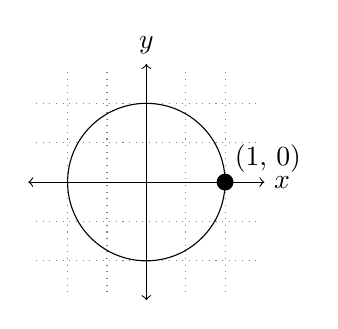
\begin{tikzpicture}

\draw[dotted,step=0.5cm, color=gray] (-1.4,-1.4) grid (1.4,1.4);
\draw (0,0) circle (1cm);
\draw[<->] (-1.5,0)--(1.5,0) node[right]{$x$};
\draw[<->] (0,-1.5)--(0,1.5) node[above]{$y$};

\draw[fill=black] (1, 0) circle (0.1cm) node[above right]{(1, 0)};
\end{tikzpicture}

\subsection{Examples}
\begin{enumerate}
\item Show the point $P\left( \frac{\sqrt{3}}{3}, \frac{\sqrt{6}}{3} \right)$ is on the unity circle. \\
{\color{blue} Sub into the equation:
\begin{align*}
\left( \frac{\sqrt{3}}{3} \right)^2 + \left( \frac{\sqrt{6}}{3} \right)^2 = \frac{3}{9} + \frac{6}{9} = 9/9 = 1
\end{align*}
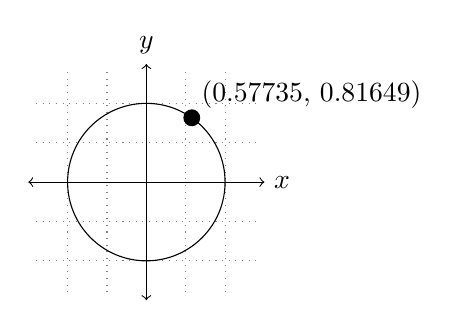
\begin{tikzpicture}

\draw[dotted,step=0.5cm, color=gray] (-1.4,-1.4) grid (1.4,1.4);
\draw (0,0) circle (1cm);
\draw[<->] (-1.5,0)--(1.5,0) node[right]{$x$};
\draw[<->] (0,-1.5)--(0,1.5) node[above]{$y$};

\draw[fill=black] (.57735, .81649) circle (0.1cm) node[above right]{(0.57735, 0.81649)};
\end{tikzpicture}
}
\item What is the $y$ coordinate for the point $P(\sqrt{3}/2, y)$?
{\color{blue} Sub into equation and get
\begin{align*}
\left( \frac{\sqrt{3}}{2} \right)^2 + y^2 = 1 \Rightarrow
y^2 = 1 - \frac{3}{4} \Rightarrow
y = \pm \frac{1}{2}
\end{align*}
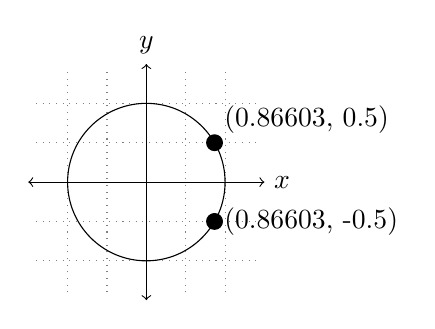
\begin{tikzpicture}

\draw[dotted,step=0.5cm, color=gray] (-1.4,-1.4) grid (1.4,1.4);
\draw (0,0) circle (1cm);
\draw[<->] (-1.5,0)--(1.5,0) node[right]{$x$};
\draw[<->] (0,-1.5)--(0,1.5) node[above]{$y$};

\draw[fill=black] (.86603, 0.5) circle (0.1cm) node[above right]{(0.86603, 0.5)};
\draw[fill=black] (.86603, -0.5) circle (0.1cm) node[right]{(0.86603, -0.5)};
\end{tikzpicture}
}
\end{enumerate}

\section{Terminal Points}
Distance $t$ on the unit circle.
Starting at $(1, 0)$, move counterclockwise if $t$ is positive, and clockwise if $t$ is negative.
One revolution is $2\pi$.
\begin{figure}[h!]
\centering
\begin{subfigure}[t]{0.24\textwidth}
\centering
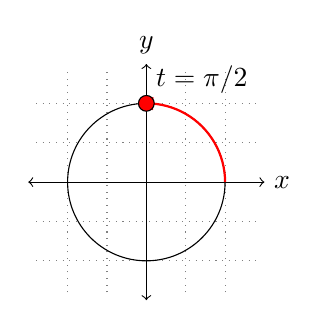
\begin{tikzpicture}

\draw[dotted,step=0.5cm, color=gray] (-1.4,-1.4) grid (1.4,1.4);
\draw (0,0) circle (1cm);
\draw[<->] (-1.5,0)--(1.5,0) node[right]{$x$};
\draw[<->] (0,-1.5)--(0,1.5) node[above]{$y$};

\draw [red, thick, ->, domain=0:90] plot ({cos(\x)}, {sin(\x)});
\draw[fill=red] (0,1) circle (0.1cm) node[above right]{$t = \pi/2$};
\end{tikzpicture}
\end{subfigure}
\begin{subfigure}[t]{0.24\textwidth}
\centering
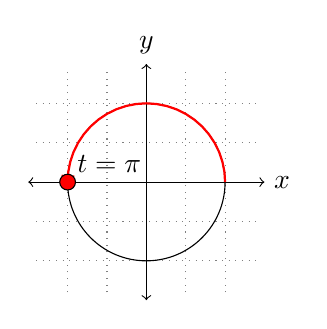
\begin{tikzpicture}

\draw[dotted,step=0.5cm, color=gray] (-1.4,-1.4) grid (1.4,1.4);
\draw (0,0) circle (1cm);
\draw[<->] (-1.5,0)--(1.5,0) node[right]{$x$};
\draw[<->] (0,-1.5)--(0,1.5) node[above]{$y$};

\draw [red, thick, ->, domain=0:180] plot ({cos(\x)}, {sin(\x)});
\draw[fill=red] (-1, 0) circle (0.1cm) node[above right]{$t = \pi$};
\end{tikzpicture}
\end{subfigure}
\begin{subfigure}[t]{0.24\textwidth}
\centering
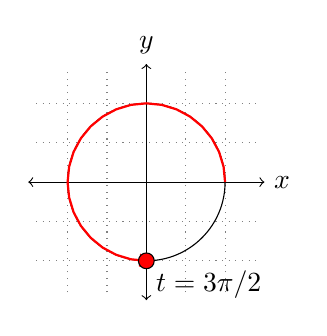
\begin{tikzpicture}

\draw[dotted,step=0.5cm, color=gray] (-1.4,-1.4) grid (1.4,1.4);
\draw (0,0) circle (1cm);
\draw[<->] (-1.5,0)--(1.5,0) node[right]{$x$};
\draw[<->] (0,-1.5)--(0,1.5) node[above]{$y$};

\draw [red, thick, ->, domain=0:270] plot ({cos(\x)}, {sin(\x)});
\draw[fill=red] (0, -1) circle (0.1cm) node[below right]{$t = 3\pi/2$};
\end{tikzpicture}
\end{subfigure}
\begin{subfigure}[t]{0.24\textwidth}
\centering
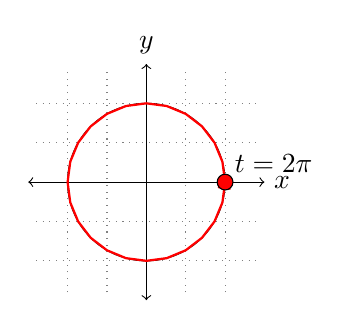
\begin{tikzpicture}

\draw[dotted,step=0.5cm, color=gray] (-1.4,-1.4) grid (1.4,1.4);
\draw (0,0) circle (1cm);
\draw[<->] (-1.5,0)--(1.5,0) node[right]{$x$};
\draw[<->] (0,-1.5)--(0,1.5) node[above]{$y$};

\draw [red, thick, ->, domain=0:360] plot ({cos(\x)}, {sin(\x)});
\draw[fill=red] (1, 0) circle (0.1cm) node[above right]{$t = 2\pi$};
\end{tikzpicture}
\end{subfigure}
\end{figure}

\subsection{Examples}
Find terminal points for 
\begin{enumerate}
\item $t = 3\pi$ {\color{blue} (-1, 0)}
\item $t = -\pi$ {\color{blue} (-1, 0)}
\item $t = -\pi/2$ {\color{blue} (0, -1)}
\item $t = \pi/4$ {\color{blue} $(\frac{\sqrt{2}}{2}, \frac{\sqrt{2}}{2})$}
\item $t = \pi/6$ {\color{blue} $(\frac{\sqrt{3}}{2}, \frac{1}{2})$}
\item $t = \pi/3$ {\color{blue} $(\frac{1}{2}, \frac{\sqrt{3}}{2})$}
\item $t = -\pi/4$ {\color{blue} $(\frac{\sqrt{2}}{2}, -\frac{\sqrt{2}}{2})$}
\item $t = -5\pi/6$ {\color{blue} $(-\frac{\sqrt{3}}{2}, -\frac{1}{2})$}
\end{enumerate}

\section{The Reference Number}
Given a $t \in \R{}$, the \textbf{reference number} $\bar{t}$ associated with $t$ is the shortest distance along the unit circle between the terminal point determined by $t$ and the $x$-axis.
Note: $\bar{t}$ always positive. \\
Can use ref. \# to find terminal points
\begin{enumerate}
\item Find the ref. \# $\bar{t}$ 
\item Find the terminal point $Q(a, b)$ determined by $\bar{t}$
\item The terminal point of $t$ is $P(\pm a, \pm b)$ where signs are determined by quadrant.
\end{enumerate}

\subsection{Examples}
\begin{enumerate}
\item Find reference numbers for 
\begin{enumerate}
\item $t = 5\pi/6$ {\color{blue} $\bar{t} = \pi/6$}
\item $t = -2\pi/3$ {\color{blue} $\bar{t} = \pi/3$}
\item $t = 5.80$ {\color{blue} $\bar{t} = 2\pi - 5.80 \approx 0.48$}
\end{enumerate}
\item Find terminal point for
\begin{enumerate}
\item $t = 5\pi/6$ {\color{blue} $(-\sqrt{3}/2, 1/2)$}
\item $t = -2\pi/3$ {\color{blue} $(-1/2, -\sqrt{3}/2)$}
\item $t = 29\pi/6$ {\color{blue} $t = 4\pi + 5\pi/6$ so $\bar{t} = \pi/6$ answer above}
\end{enumerate}
\end{enumerate}


\end{document}